\documentclass[12pt,a4paper,oneside]{paper}
%TC:ignore
% ################################################################################
% 
%       INSTRUCTIONS, PLEASE READ BEFORE IF YOU INTEND TO MODIFY THIS FILE
% 
% ################################################################################
% For the most part, you should not change this file. In particular, the format 
% should not be changed. However, depending on what you want you might need to
% use additional packages (and possibly remove old ones that may be incompatible.
% Do that at your own discretion.
% ################################################################################

% Encoding and Language
\usepackage[utf8]{inputenc} % Changed from utf8x to utf8
\usepackage{csquotes}
\usepackage[main=english]{babel}
\usepackage{iflang}

% Font Configurations
\renewcommand{\rmdefault}{phv}
\renewcommand{\sfdefault}{phv}
\def\FontLn{% 16 pt normal
  \usefont{T1}{phv}{m}{n}\fontsize{14pt}{14pt}\selectfont}
\def\FontLb{% 16 pt bold
  \usefont{T1}{phv}{b}{n}\fontsize{14pt}{14pt}\selectfont}
\def\FontMn{% 14 pt normal
  \usefont{T1}{phv}{m}{n}\fontsize{12pt}{12pt}\selectfont}
\def\FontMb{% 14 pt bold
  \usefont{T1}{phv}{b}{n}\fontsize{12pt}{12pt}\selectfont}
\def\FontSn{% 12 pt normal
  \usefont{T1}{phv}{m}{n}\fontsize{10pt}{10pt}\selectfont}

% Font Encoding
\usepackage[T1]{fontenc}

% Page Geometry
\usepackage{geometry}	
\geometry{verbose,tmargin=2cm,bmargin=1.7cm,lmargin=1.6cm,rmargin=1.9cm}
\usepackage{multirow}
\usepackage{multicol}

% Graphics and Figures
\usepackage{graphicx}
\usepackage{subfigure}
\usepackage{subfigmat}

%Colors
\usepackage{xcolor}

% Mathematics and Theorems
\usepackage{amsmath}
\usepackage{bm}
\usepackage{amsthm}
\usepackage{amsfonts}
\usepackage{dcolumn}
\usepackage{indentfirst}
\usepackage{dsfont}

% Comments and Verbatim
\usepackage{verbatim}

% Hyperlinks
\usepackage[pdftex]{hyperref}
\hypersetup{
    colorlinks=true,
    linkcolor=blue,
    anchorcolor=black,
    citecolor=cyan,
    filecolor=black,
    menucolor=black,
    urlcolor=teal,
    bookmarksopen=true,
    bookmarksnumbered=true
}

% Captions and References
\usepackage[figure,table]{hypcap}
\usepackage[format=plain]{caption}
\DeclareCaptionFont{georgia}{\small\fontseries{n}\fontfamily{georgia}\selectfont}
\captionsetup{labelfont=georgia,font=georgia}

% Algorithm packages
% \usepackage{algorithm2e}
\usepackage{algorithm}
\usepackage{algpseudocode}
\usepackage{float} % For [H] placement

% Line Spacing
\usepackage{setspace}
\renewcommand{\baselinestretch}{1.2}

% Bibliography
\usepackage[backend=biber,style=apa]{biblatex}

% Index
\usepackage{makeidx}
\makeindex

% Acronyms
\usepackage[printonlyused]{acronym}

% Lipsum (for placeholder text)
\usepackage{lipsum}

% Cleveref (for clever references)
\usepackage[\IfLanguageName{english}{english}{portuguese}]{cleveref}
\Crefname{equation}{Eq.}{Eqs.}

% Custom Commands
\newcommand{\gray}[1]{\textcolor{gray}{#1}}

% Equation Numbering
\renewcommand{\theequation}{{\fontseries{n}\fontfamily{georgia}\selectfont\arabic{equation}}}

% Section and Subsection Fonts
\sectionfont{\Large\bfseries\fontfamily{lmss}\selectfont}
\subsectionfont{\large\bfseries\fontfamily{lmss}\selectfont}
%TC:endignore

\addbibresource{bibliography.bib}
\begin{document}
\pagestyle{plain}


% Title
\def\title {Homework Assignment 4}

% Input the cover
\thispagestyle {empty}
\begin{center}
\begin{minipage}[c][5cm][t]{\textwidth}
\begin{center}

\includegraphics[width=10cm]{./logo/logoUvA_en.pdf}
\end{center}

\end{minipage}
\begin{minipage}[t][10cm][c]{\textwidth}
\centering
{\FontMb University of Amsterdam} \\
\paragraph{}
\centering
{\FontLb\Huge \title{}}
\paragraph{}
\centering
{\FontMb Machine Learning I} \\
\paragraph{}
{\FontMb 2024}
\end{minipage}

\begin{minipage}[c][2cm][c]{\textwidth}
\centering
{\FontLn }
\end{minipage}
\begin{minipage}[c][2cm][c]{\textwidth}
\centering
\end{minipage}
\begin{minipage}[c][8cm][c]{\textwidth}
\centering
{\FontMb
Pedro M. P. Curvo\\
15713725}
\end{minipage}

\end{center} 
\cleardoublepage
\fontfamily{cmr}\selectfont
\setcounter{page}{0}
\tableofcontents
\newpage

\small

\section{Maximum Margin Classifier}

\subsection*{a)}

By applying the transformation $\phi(x)$ to the dataset, the points are mapped onto a circumference in the transformed
space, with the boundary alternating between the \textit{red} and \textit{blue} points. This transformation can be
decomposed into $\phi(x) = \phi_1(x) \circ \phi_2(x)$, where $\phi_1(x)$ maps the points as $\phi_1(x) = (x^{(1)} - x^{(2)}, x^{(1)} - x^{(2)})$,
projecting the data along the principal component $[1, -1]$ and forming a diagonal where the points alternate between
the red and blue regions in a periodic way. The second transformation, $\phi_2(x)$, applies trigonometric functions,
$\phi_2(x) = (\cos(x^{(1)}), \sin(x^{(2)}))$, which maps the points onto a circular path, resulting in the points
alternating between the red and blue regions along the circumference.

\newpage
\subsection*{b)}

The decision boundary is defined by the equation:

\begin{align*}
    y(x) = \bm{w}^T \phi(x) + b = w_0 \cos(x^{(1)} - x^{(2)}) + w_1 \sin(x^{(1)} - x^{(2)}) - b
\end{align*}

If $y(x) = 0$, then the decision boundary is defined by the equation:

\begin{align*}
    y(x) &= 0 \\
    w_0 cos(x^{(1)} - x^{(2)}) + w_1 \sin(x^{(1)} - x^{(2)}) - b &= 0 \\
    \sin(x^{(1)} - x^{(2)}) &= -\frac{w_0}{w_1} \cos(x^{(1)} - x^{(2)}) + \frac{b}{w_1} \\
\end{align*}

In the new space, $\phi(x)^{(1)} = \cos(x^{(1)} - x^{(2)})$ and $\phi(x)^{(2)} = \sin(x^{(1)} - x^{(2)})$, so this becomes:

\begin{align*}
    y(x) &= 0 \\
    \phi(x)^{(2)} &= -\frac{w_0}{w_1} \phi(x)^{(1)} + \frac{b}{w_1} \\
\end{align*}

Which is the equation of a straight line in the new space, hence the $w$ is the vector that controls the slope
of the decision boundary, and $b$ is the bias term that controls the offset of the decision boundary shifting it
up or down.

\newpage
\subsection*{c)}

By introducing the Lagrange multipliers $\lambda_n$ for the first constraint and $\mu_n$ for the second constraint, we can write the primal Lagrangian as:

\begin{align*}
    \mathcal{L} (w, b, \lambda, \mu) = \frac{1}{2} ||w||^2 + C \sum_{n=1}^{N} \xi_n - \sum_{n=1}^{N} \lambda_n \left( t_n (\bm{w}^T \bm{\phi(x_n)} + b) - 1 + \xi_n \right) - \sum_{n=1}^{N} \mu_n \xi_n
\end{align*}

With:

\begin{align*}
    \xi_n \geq 0, \quad \lambda_n \geq 0, \quad \mu_n \geq 0
\end{align*}

\newpage
\subsection*{d)}

The KKT conditions for the primal problem are:

\textbf{Primal Feasibility:}

\begin{align*}
    t_n (\bm{w}^T \bm{\phi(x_n)} + b) \geq 1 - \xi_n, \quad \forall n \\
    \xi_n \geq 0 \quad \forall n
\end{align*}

\textbf{Dual Feasibility:}

\begin{align*}
    \lambda_n \geq 0 \\
     \mu_n \geq 0
\end{align*}

\textbf{Complementary Slackness:}

\begin{align*}
    \lambda_n \left( t_n (\bm{w}^T \bm{\phi(x_n)} + b) - 1 + \xi_n \right) = 0, \quad \forall n \\
    \mu_n \xi_n = 0, \quad \forall n
\end{align*}

With this we have 6 KKT conditions per point, 3 for each constraint condition in the primal problem. So, 
in the overall problem we have $6N$ KKT conditions.

\newpage
\subsection*{e)}

To derive the dual Lagrangian $\tilde{\mathcal{L} }(\lambda)$, we need to find the stationary conditions for the primal Lagrangian $\mathcal{L} (w, b, \lambda, \mu)$
by taking the derivatives with respect to $w$, $b$ and $\xi_n$ and setting them to zero, to find the optima of the primal problem.

\begin{align*}
    \frac{\partial \mathcal{L} }{\partial w} &= 0 \\
    0 &= \frac{\partial}{\partial w} \frac{1}{2} ||w||^2 + C \sum_{n=1}^{N} \xi_n - \sum_{n=1}^{N} \lambda_n \left( t_n (\bm{w}^T \bm{\phi(x_n)} + b) - 1 + \xi_n \right) - \sum_{n=1}^{N} \mu_n \xi_n \\
    0 &= w - \sum_{n=1}^{N} \lambda_n t_n \bm{\phi(x_n)} \\
    w &= \sum_{n=1}^{N} \lambda_n t_n \bm{\phi(x_n)}
\end{align*}

\begin{align*}
    \frac{\partial \mathcal{L} }{\partial b} &= 0 \\
    0 &= \frac{\partial}{\partial b} \frac{1}{2} ||w||^2 + C \sum_{n=1}^{N} \xi_n - \sum_{n=1}^{N} \lambda_n \left( t_n (\bm{w}^T \bm{\phi(x_n)} + b) - 1 + \xi_n \right) - \sum_{n=1}^{N} \mu_n \xi_n \\
    0 &= -\sum_{n=1}^{N} \lambda_n t_n \\
    0 &= \sum_{n=1}^{N} \lambda_n t_n
\end{align*}

\begin{align*}
    \frac{\partial \mathcal{L} }{\partial \xi_n} &= 0 \\
    0 &= \frac{\partial}{\partial \xi_n} \frac{1}{2} ||w||^2 + C \sum_{n=1}^{N} \xi_n - \sum_{n=1}^{N} \lambda_n \left( t_n (\bm{w}^T \bm{\phi(x_n)} + b) - 1 + \xi_n \right) - \sum_{n=1}^{N} \mu_n \xi_n \\
    0 &= C - \lambda_n - \mu_n \\
    \lambda_n &= C - \mu_n
\end{align*}

Now by substituting the values into the primal Lagrangian, we can obtain the dual Lagrangian $\tilde{\mathcal{L} }(\lambda)$:

\begin{align*}
    \tilde{\mathcal{L} }(\lambda) &= \frac{1}{2} \bm{w}^T \bm{w} + C \sum_{n=1}^{N} \xi_n - \sum_{n=1}^{N} \lambda_n \left( t_n (\bm{w}^T \bm{\phi(x_n)} + b) - 1 + \xi_n \right) - \sum_{n=1}^{N} \mu_n \xi_n \\
    &= \bm{w}^T \left( \frac{1}{2} \bm{w} - \sum_{n=1}^{N} \lambda_n t_n \bm{\phi(x_n)} \right) + C \sum_{n=1}^{N} \xi_n - \sum_{n=1}^{N} \lambda_n t_n b + \sum_{n=1}^{N} \lambda_n - \sum_{n=1}^{N} \lambda_n \xi_n - \sum_{n=1}^{N} \mu_n \xi_n \\
    &= \bm{w}^T \left( \frac{1}{2} \bm{w} - \bm{w} \right) - b \sum_{n=1}^{N} \lambda_n t_n + \sum_{n=1}^{N} \lambda_n + C \sum_{n=1}^{N} \xi_n - \sum_{n=1}^{N} \lambda_n \xi_n - \sum_{n=1}^{N} \mu_n \xi_n \\
    &= -\frac{1}{2} \bm{w}^T \bm{w} + \sum_{n=1}^{N} \lambda_n + C \sum_{n=1}^{N} \xi_n - \sum_{n=1}^{N} (\lambda_n + \mu_n) \xi_n \quad \text{, since $\sum_{n=1}^{N} \lambda_n t_n = 0$} \\
    &= -\frac{1}{2} \bm{w}^T \bm{w} + \sum_{n=1}^{N} \lambda_n \quad \text{ , since $\lambda_n = C - \mu_n$} \\
    &= -\frac{1}{2} \sum_{n=1}^{N} \lambda_n t_n \bm{\phi(x_n)}^T \sum_{m=1}^{N} \lambda_m t_m \bm{\phi(x_m)} + \sum_{n=1}^{N} \lambda_n \quad \text{, since $w = \sum_{n=1}^{N} \lambda_n t_n \bm{\phi(x_n)}$} \\
    &= -\frac{1}{2} \sum_{n=1}^{N} \sum_{m=1}^{N} \lambda_n \lambda_m t_n t_m \bm{\phi(x_n)}^T \bm{\phi(x_m)} + \sum_{n=1}^{N} \lambda_n
\end{align*}
With the remaining constraints of the dual problem:

\begin{align*}
    0 \leq \lambda_n \leq C, \quad \forall n \\
    \sum_{n=1}^{N} \lambda_n t_n = 0
\end{align*}

The dual optimization problem is then:

\begin{align*}
    {\lambda}^* = arg\min_{\lambda} \tilde{\mathcal{L}} (\lambda) = arg\min_{\lambda} \left( -\frac{1}{2} \sum_{n=1}^{N} \sum_{m=1}^{N} \lambda_n \lambda_m t_n t_m \bm{\phi(x_n)}^T \bm{\phi(x_m)} + \sum_{n=1}^{N} \lambda_n \right)
\end{align*}

Subject to the constraints presented above.

\newpage
\subsection*{f)}

The kernel function $\kappa (x, x')$ in the dual Lagrangian is given by:

\begin{align*}
    \kappa (x_n, x_m) &= \bm{\phi(x_n)}^T \bm{\phi(x_m)} \\
    &= \cos(x_n^{(1)} - x_n^{(2)}) \cos(x_m^{(1)} - x_m^{(2)}) + \sin(x_n^{(1)} - x_n^{(2)}) \sin(x_m^{(1)} - x_m^{(2)}) \\
    &= \cos((x_n^{(1)} - x_n^{(2)}) - (x_m^{(1)} - x_m^{(2)})) \quad \text{, by the trigonometric identity} \\
\end{align*}

\newpage
\subsection*{g)}

To classify a new point $x^\ast$, we need to evaluate $y(x^\ast)$, but since we have the dual solution $\lambda_n$, we can write $y(x^\ast)$ as:

\begin{align*}
    y(x^\ast) &= \bm{w}^T \bm{\phi(x^\ast)} + b \\
    &= \sum_{n=1}^{N} \lambda_n t_n \kappa (x_n, x^\ast_m) + b \quad \text{, by the definition of $w$ in the dual solution} \\
\end{align*}

Where $\kappa (x_n, x_m)$ is the kernel function $\bm{\phi(x_n)}^T \bm{\phi(x_m)}$.

To evaluate the point we can just evaluate the sign of $y(x^\ast)$, if $y(x^\ast) > 0$, then the point is classified as $t = 1$, if $y(x^\ast) < 0$, then the point is classified as $t = -1$.
We can do this because we already know the $\lambda_n$ and $b$ values, and we can evaluate the kernel function $k(x_n, x^\ast_m)$ for all the support vectors.

\newpage
\subsection*{h)}

For a new prediticion we have that:

\begin{align*}
    y(x) &= \sum_{n=1}^{N} \lambda_n t_n \kappa (x_n, x_m) + b
\end{align*}

with 

\begin{align*}
    0 \leq \lambda_n \leq C, \quad \forall n \quad \text{and} \quad \sum_{n=1}^{N} \lambda_n t_n = 0
\end{align*}

And from the KKT conditions we have that:

\begin{align*}
    \lambda_n \geq 0, \quad \mu_n \geq 0 \\
    \lambda_n \left( t_n (\bm{w}^T \bm{\phi(x_n)} + b) - 1 + \xi_n \right) = 0, \quad \mu_n \xi_n = 0 \\
    t_n (\bm{w}^T \bm{\phi(x_n)} + b) \geq 1 - \xi_n, \quad \xi_n \geq 0
\end{align*}

Now, with this constraints and by the way we define the problem, than
if $\lambda_n > 0$ we have a support vector that is on the region that is defined by the margin and the decision boundary.

Now, if $\lambda_n = 0$, then $t_n y(x_n) = 1 - \xi_n$. With this we can conclude several things:

\begin{itemize}
    \item If $\lambda_n < C$, then $\mu_n > 0$ because $\lambda_n = C - \mu_n$. Meaning that $\xi_n = 0$, since $\mu_n \xi_n = 0$.
Since $\xi_n$ defines distance from the margin, if $\xi_n = 0$, then the point is on the margin.
    \item If $\lambda_n = C$, then $\mu_n = 0$ because $\lambda_n = C - \mu_n$. Meaning that $\xi_n > 0$, since $\mu_n \xi_n = 0$.
Now, by the definition of $\xi_n$, if $\xi_n > 1$, then the point is on the wrong side of the margin, and is misclassified.
If $\xi_n \leq 1$, then the point is within the margin and is correctly classified.
\end{itemize}

With this we can resume in the following:

\begin{itemize}
    \item Outside the margin, correctly classified: $\lambda_n = 0$
    \item On the margin (support vector), correctly classified: $0 < \lambda_n < C$, $\mu_n > 0$, $\xi_n = 0$
    \item Inside the margin, correctly classified: $\lambda_n = C$, $\mu_n = 0$, $0 \leq \xi_n \leq 1$
    \item Inside the margin, misclassified: $\lambda_n = C$, $\mu_n = 0$, $\xi_n > 1$
\end{itemize}

\newpage
\subsection*{i)}

To find the optimal values for the dual variables $\mu_n$ given the optimal values for the dual variables $\lambda_n$, we can use the the previous shown conditions that: 

\begin{align*}
    \lambda_n = C - \mu_n
\end{align*}

With this we can find the optimal values for $\mu_n$.

Now, by using the KKT conditions, we can solve for the primal variables $w$, $b$ and $\xi_n$:

\begin{align*}
    w &= \sum_{n=1}^{N} \lambda_n t_n \bm{\phi(x_n)} \\
    b &= \frac{1}{N} \sum_{n=1}^{N} \left( t_n - \sum_{m=1}^{N} \lambda_m t_m \kappa (x_m, x_n) \right) \quad \text{, by inverting the problem and isolating $b$} \\
    \xi_n &= \max(0, 1 - t_n (\bm{w}^T \bm{\phi(x_n)} + b))
\end{align*}

Where in $b$, we are taking the average of the support vectors $N$ just to ensure that we are getting a good estimate of the bias, 
since the program solving for the dual problem might not be able to find the exact value of $b$.

In $\xi_n$ we are taking the maximum of $0$ and $1 - t_n (\bm{w}^T \bm{\phi(x_n)} + b)$, since this shows if the margin
is being violated or not, i.e., if the points is correctly classified and lies on/or outside the margin
then $\xi_n = 0$. For points misclassified or inside the margin, then $\xi_n > 0$. Now, according to the restritions,
$\xi_n \leq 1 - t_n (\bm{w}^T \bm{\phi(x_n)} + b)$, so taking the maximum of $0$ and $1 - t_n (\bm{w}^T \bm{\phi(x_n)} + b)$ ensures that
the $\xi_n$ is within the bounds.

\newpage
\subsection*{j)}

\textbf{Dataset 1:}

This dataset looks like the XOR function but rotated, so first we can rotate the dataset by 45 degrees counter clockwise:

\begin{align*}
    \begin{bmatrix}
        \phi_1(x)^{(1)} \\
        \phi_1(x)^{(2)}
    \end{bmatrix} =
    \begin{bmatrix}
        \cos(45) & -\sin(45) \\
        \sin(45) & \cos(45)
    \end{bmatrix}
    \begin{bmatrix}
        x^{(1)} \\
        x^{(2)}
    \end{bmatrix}
    =
    \begin{bmatrix}
        \frac{1}{\sqrt{2}} & -\frac{1}{\sqrt{2}} \\
        \frac{1}{\sqrt{2}} & \frac{1}{\sqrt{2}}
    \end{bmatrix}
    \begin{bmatrix}
        x^{(1)} \\
        x^{(2)}
    \end{bmatrix}
    =
    \begin{bmatrix}
        \frac{x^{(1)} - x^{(2)}}{\sqrt{2}} \\
        \frac{x^{(1)} + x^{(2)}}{\sqrt{2}}
    \end{bmatrix}
\end{align*}

Then, we can see that the \textit{blue} points, in the new space, have the characteristic that $x^{(1)} \cdot x^{(2)} < 0$, and the \textit{red} points have the characteristic that $x^{(1)} \cdot x^{(2)} > 0$, because
they are going to be in different quadrants.
So we can just apply the transformation $\phi_2(x) = ((x^{(1)} \cdot x^{(2)}), (x^{(1)} \cdot x^{(2)}))$ to the dataset and then they will be separated by a line
passing through quadrants 2 and 4.

The total trasnformation is then:

\begin{align*}
    \phi(x) = (\frac{(x^{(1)} - x^{(2)})(x^{(1)} + x^{(2)})}{2}, \frac{(x^{(1)} - x^{(2)})(x^{(1)} + x^{(2)})}{2})
\end{align*}

\textbf{Dataset 2:}

Looking into the dataset, we can see some periodicity in the direction $[1, 1]$ but with varying amplitude, so we can apply
first a trasnformation that projects the data onto that component $[1, 1]$ such as $\phi_1(x) = (x^{(1)} + x^{(2)}, x^{(1)} + x^{(2)})$.
Then we can apply a transformation that maps the data onto the function $\frac{\sin x}{x}$, since the periodicity
looks like the function and the width can be estimated. With that the total transformation is:

\begin{align*}
    \phi(x) = \left( (x^{(1)} + x^{(2)}), \frac{\sin(x^{(1)} + x^{(2)})}{x^{(1)} + x^{(2)}} \right)
\end{align*}

Looking something like: 

\begin{figure}[H]
    \centering
    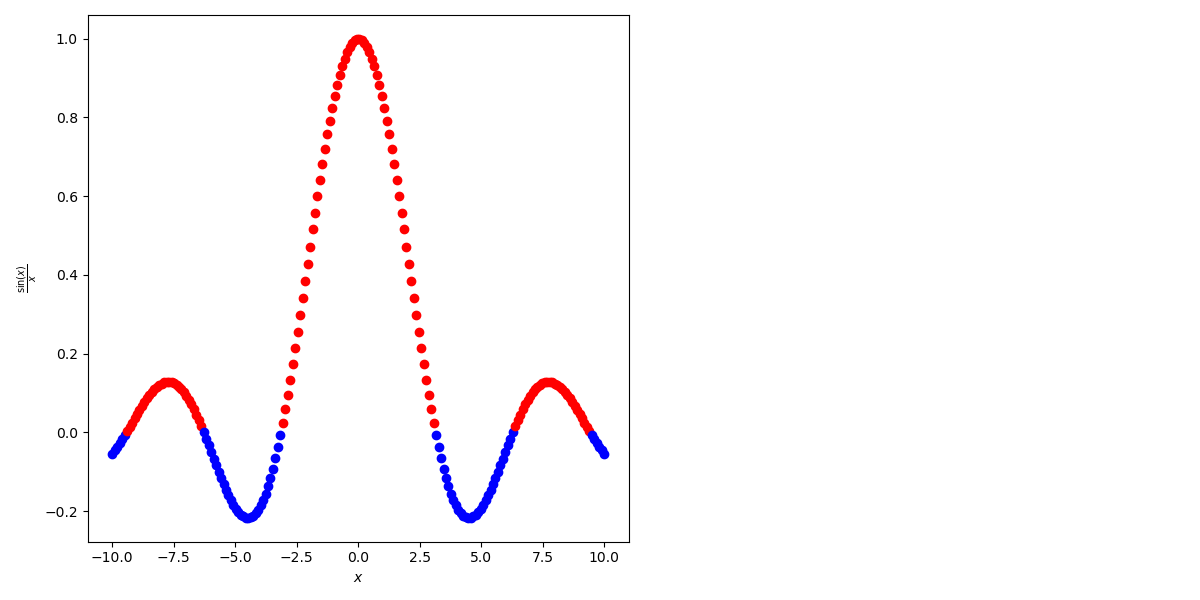
\includegraphics[width=0.8\textwidth]{sin_x_over_x.png}
\end{figure}

To be in mind that constant values of the function, such as the constants for dilation and translation are not defined,
but can be estimated by the data.
Moreover, each periodic signal can be expressed as a fourier series, so we could also use a sum of sins and cosines to map the
periodicity of the data as the second coordinate of the transformation.

\textbf{Dataset 3:}

For this dataset there are several approaches we could try. 
First, we can rotate the dataset by 45 degrees counter clockwise
and apply the transformation from the previous dataset $sin(x)/x$ to map the data to a 2D space where the data is linearly separable.
Besides that, after the rotation we can also apply a sum of sins and cosines since its periodicity can be mapped by a fourier series.
Hence, one possible solution could be the following transformation:

\begin{align*}
    \phi(x) = \left( \frac{(x^{(1)} - x^{(2)})(x^{(1)} + x^{(2)})}{2}, \frac{\sin\left(\frac{(x^{(1)} - x^{(2)})(x^{(1)} + x^{(2)})}{2}\right)}{\frac{(x^{(1)} - x^{(2)})(x^{(1)} + x^{(2)})}{2}} \right)
\end{align*}

Another solution, since the data looks like two spirals intertwined in a 3D space, but seen from above, we could try to first estimate the radius of the spiral, the angle of each point relative to the center of the spiral, and width of the spiral
by the distance between "wavelengths". With this we can create the typical 3D space of a spiral, where the axis are given by $cos(\theta)$, $sin(\theta)$ and $\theta$.
Now, we could simply apply the function $\arccos$ to one of the trigonometric axis to map the data to a any 2D space where this is one axis.
Why this function? So the spirals are intertwined, but not overlapping, meaning that the angle of one is shifted by a constant value relative to the other, so
the $\arccos$ function could map the data to a 2D space where the spirals are linearly separable, because it would look something like $\theta$ for one spiral and $\theta + \delta$ for the other.

Due to the complexity of what was presented above, an alternative would be to use a RBF kernel, since it can
map the data into a space where it is linearly separable, due to the periodicity of the data.


\clearpage

\appendix


\newpage
\printbibliography

\end{document}

